\section{Consistency of Capitalization Tables - Alloy Model}
\label{ch:transaction-tracing}
\label{sec:transaction-tracing}

We developed an Alloy model based on the OCF that encompasses the OCF structure and the semantics of transactions permitted in financial systems.
In this section, we explore the portion of the Alloy model that ensures the consistency of \glspl{transaction} that affect capitalization tables. 

A \gls{capitalization-table} tracks the ownership stakes and capital structure of a company. The \glspl{transaction} that typically affect a \gls{capitalization-table} include \glspl{issuance}, cancellations, and transfers of  \glspl{security} 
%
(model overview in Fig.~\ref{fig:metamodel}).

\begin{figure}[!h]
	\centering
	\fbox{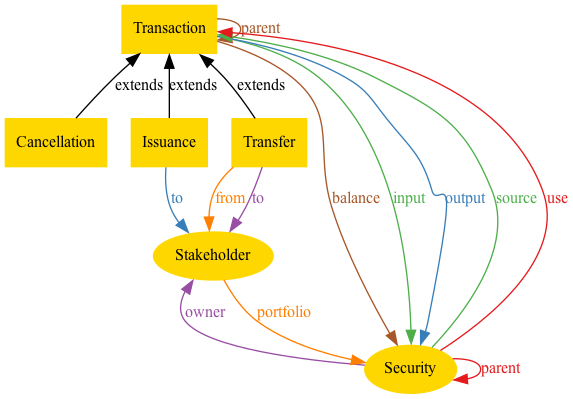
\includegraphics[width=0.7\textwidth]{images/metamodel5.png}}
	\caption{Transaction tracing metamodel: 
	Rendered by the Alloy Analyzer \label{fig:metamodel}}
\end{figure}

%\section{Introduction}

A \gls{capitalization-table} is built as new \glspl{transaction} are recorded. The Open Cap Table format proposes a ''transaction tracing model'' in which \glspl{security} are identified with unique identifiers and \glspl{transaction} refer to those identifiers when issuing, canceling, or transferring \glspl{security}.

The purpose of the transaction tracing model is to provide auditable \glspl{security} traceability. The Alloy model then needs to conform to the requirements for a consistent model for capitalization tables and enforce certain properties.

\subsection{Expected Properties}
\label{sec:exp-properties}

%Let's begin by defining the expected properties that the model must hold. 
The following properties must be satisfied regarding the graph of \glspl{security} and \glspl{transaction}:


\begin{description}
	\item [P1:] All \glspl{security} can be traced back to an Issuance.
	\item [P2:] All \glspl{transaction} can be traced back to an Issuance.
	\item [P3:] There can be no cycles in the \gls{security} hierarchy. This guarantees that every \gls{security} can be traced back to a root security.
	\item [P4:] There can be no cycles in the transaction hierarchy. This guarantees that every transaction can be traced back to a root transaction.
\end{description}

Additionally, the following accounting identity-related properties are defined:

\begin{description}
	\item [P5:] The number of shares in circulation should be less than or equal to the number of shares issued.
	\item [P6:] No \glspl{security} can have a negative number of shares.
	\item [P7:] The sum of shares in all portfolios should be equal to the number of shares issued minus the number of shares cancelled.
\end{description}

The properties above cannot be expressed in JSON Schema, but are expected for a consistent model of capitalization tables. The Alloy model must ensure that these properties hold, as checked by the Alloy Analyzer.

%We will give precise Alloy predicates for each of the properties.

\subsection{The Alloy Model}

This section presents the main elements of the model, illustrating each signature, predicate, and fact with a code excerpt.

\subsubsection{Securities and Transactions.}

The first elements consists of signatures for \glspl{security} and \glspl{transaction}, together with opening of the ordering and graph modules for both signatures, as they will form a complex structure that can be traced back to issuances (Listing \ref{list:security-transitions}).

\begin{listing}[!h]
 \begin{multicols}{2}
	\begin{minted}[fontsize=\footnotesize]
     {alloy}
open util/ordering[Security]
open util/ordering[Transaction]

open util/graph[Security]
open util/graph[Transaction]

sig Security {
    shares : Int,
    source : one Transaction,
    use : lone Transaction,
    parent : lone Security,
    owner : Stakeholder
} {
    nonneg[shares]
}

abstract sig Transaction {
    shares : Int,
    input : lone Security,
    output : lone Security,
    balance : lone Security,
    parent : lone Transaction
} {
    pos[shares]
}
fact {
    use = ~input
}
fact {
    source = ~(output + balance)
}
\end{minted}
\end{multicols}
	\caption{Security and Transaction Signatures and Constraints
    \label{list:security-transitions}
    }
\end{listing}

The \verb|Transaction| signature is given abstract because a \verb|Transaction| is never instantiated directly; they may have different types of \glspl{transaction}, such as issuances, cancellations, and transfers. Those types of \glspl{transaction} are defined afterwards.

Two constraints are stated as facts to relate the \verb|use| and \verb|source| fields of \glspl{security} to the \verb|input| and \verb|output| fields of \glspl{transaction}. The \verb|use| field of a \gls{security} is the transaction that uses the \gls{security} as input. The \verb|source| field of a \gls{security} is the transaction that uses the \gls{security} as output.
%
%\begin{listing}[!h]
% \begin{multicols}{2}
%	\begin{minted}[fontsize=\footnotesize]
%     {alloy}
%fact {
%    use = ~input
%}
%fact {
%    source = ~(output + balance)
%}
%\end{minted}
%\end{multicols}
%	\caption{Security Use and Source
%    \label{lst:tt-alloy-security-and-transaction-signatures}}
%\end{listing}
%
The \verb|~| operator to invert the binary relations is used for \verb|input| and \verb|output| because they denote the same relation with the opposite direction.

%The three transaction types are given below.

\subsubsection{Transaction types.}

We consider three types of transaction in the model because they subsume all other more specific types of transaction. Any transaction is a composition of creation and destruction of  \glspl{security}.  Transfers, in particular, are a combination of an issuance and a cancellation (Listing \ref{lst:tt-alloy-transaction-types}).

\begin{listing}[!h]
 \begin{multicols}{2}
	\begin{minted}[fontsize=\footnotesize]
     {alloy}
sig Issuance extends Transaction {
    to : Stakeholder
} {
    no input
    no balance
    one output
    no (Transaction <: parent)
}
sig Cancellation extends Transaction {} {
    no output
    lone balance
    one input
    one (Transaction <: parent)
}
sig Transfer extends Transaction {
    from : Stakeholder,
    to : Stakeholder - from
} {
    one input
    one output
    lone balance
    one (Transaction <: parent)
}
\end{minted}
\end{multicols}
	\caption{Transaction Types}
\label{lst:tt-alloy-transaction-types}
\end{listing}

All \glspl{transaction} have \verb|parent|, \verb|input|, \verb|output|, and \verb|balance| fields, but each transaction uses only a subset of them. Additional fields, appearing after the signature, constraint the \glspl{transaction}.
%
For instance, the \verb|Issuance| transaction has a \verb|to| field stating who will own the issued security, while the \verb|Transfer| transaction has \verb|from| and \verb|to| fields stating who will transfer the \gls{security} from and to.

\subsubsection{Issuance constraints.}

The behavior of the Issuance is encoded in a single fact (Listing \ref{lst:tt-alloy-issuance-constraints}). The first line equates the number of shares of the newly issued \gls{security} to the number of the shares in the issuance, while the following lines bind other specific fields to their appropriate values.

\begin{listing}[!h]
 \begin{multicols}{2}
	\begin{minted}[fontsize=\footnotesize]
     {alloy}
fact {
    all iss : Issuance {
        eq[iss.output.shares, iss.shares]
        iss.output.source = iss
        iss.output.owner = iss.to
        iss.output in iss.to.portfolio
    }
}
\end{minted}
\end{multicols}
	\caption{Issuance Constraints}
\label{lst:tt-alloy-issuance-constraints}
\end{listing}


\subsubsection{Cancellation constraints.}

%The case for a cancellation is more complex because it must distinguish between partial and complete cancellations. This is done by comparing the number of shares in the cancellation and in the cancelled security, and giving different constraints for each case.
%%
%It is encoded in a single fact (Listing \ref{lst:tt-alloy-cancellation-constraints}).

\begin{listing}[!h]
% \begin{multicols}{2}
	\begin{minted}[fontsize=\footnotesize]
     {alloy}
fact {
    all can : Cancellation {
        lt[can.shares, can.input.shares] implies {
            // In this case, the transaction is partial.
            can.input.use = can
            can.balance.source = can
            eq[can.balance.shares, sub[can.input.shares, can.shares]]
            lt[can.input, can.balance]
            can.balance.owner = can.input.owner
            can.balance in can.input.owner.portfolio
            can.balance.parent = can.input
            can.parent = can.input.source
        } else {
            can.input.use = can
            eq[can.input.shares, can.shares]
            can.parent = can.input.source
            no can.balance            
        }
    }
}
\end{minted}
%\end{multicols}
	\caption{Cancellation Constraints}
\label{lst:tt-alloy-cancellation-constraints}
\end{listing}

The case for a cancellation is more complex because it must distinguish between partial and complete cancellations. This is done by comparing the number of shares in the cancellation and in the cancelled security, and giving different constraints for each case.
%
It is encoded in a fact (Listing \ref{lst:tt-alloy-cancellation-constraints}).

The constraints are now more detailed to ensure the balancing of shares, and the fields used to relate \glspl{security} and \glspl{transaction} in a graph.% (the \verb|parent| field, ultimately).

\subsubsection{Transfer constraints.}

Here no new logic needs to be introduced, but we now use all three fields (\verb|input|, \verb|output|, and \verb|balance|) if a partial transfer is performed (Listing \ref{lst:alloy-transfer-constraints}). %It is unfortunately more verbose.

\begin{listing}[!h]
% \begin{multicols}{2}
	\begin{minted}[fontsize=\footnotesize]
     {alloy}
fact {
    all xfer : Transfer {
        lt[xfer.shares, xfer.input.shares] implies {
            // In this case, the transaction is partial.
            xfer.input.use = xfer
            xfer.output.source = xfer
            xfer.balance.source = xfer
            eq[xfer.output.shares, xfer.shares]
            eq[xfer.balance.shares, sub[xfer.input.shares, xfer.shares]]
            lt[xfer.input, xfer.output]
            lt[xfer.input, xfer.balance]
            xfer.output.owner = xfer.to
            xfer.input.owner = xfer.from
            xfer.balance.owner = xfer.from
            xfer.from.portfolio = xfer.from.portfolio + xfer.balance
            xfer.to.portfolio = xfer.to.portfolio + xfer.output
            xfer.output.parent = xfer.input
            xfer.balance.parent = xfer.input
        } else {
            xfer.input.use = xfer
            xfer.output.source = xfer
            eq[xfer.output.shares, xfer.shares]
            eq[xfer.shares, xfer.input.shares]
            lt[xfer.input, xfer.output]
            xfer.output.owner = xfer.to
            xfer.input.owner = xfer.from            
            xfer.to.portfolio = xfer.to.portfolio + xfer.output
            xfer.output.parent = xfer.input
            no xfer.balance
        }
    }
}
\end{minted}
%\end{multicols}
	\caption{Transfer Constraints
             \label{lst:alloy-transfer-constraints}
             }
\end{listing}

We observe that the required bookkeeping in a structural Alloy model can become complex. As we add more constraints to our model, we can rely on the Alloy Analyzer to ensure that it remains consistent.

\subsection{Model Properties}

%\subsubsection{Ordering of Transaction and securities}

The hypothesis for proving the properties of the system  will be based on the ordering provided by the \verb|ordering| module for \glspl{transaction} and \glspl{security} (Listing \ref{lst:tt-alloy-ordering}). In the ordering, there is a consistent pattern for parents to always come before their children. Other auxiliary functions are defined in Appendix \ref{app:aux-functions}.


\begin{listing}[!h]
 \begin{multicols}{2}
	\begin{minted}[fontsize=\footnotesize]
     {alloy}
pred orderingOfSecurities {
    all sec : Security {
        some sec.parent implies {
            lt[sec.parent, sec]
        }
    }
}
pred orderingOfTransactions {
    all tx : Transaction {
        some tx.parent implies {
            lt[tx.parent, tx]
        }
    }
}
\end{minted}
\end{multicols}
	\caption{Ordering of Securities and \glspl{transaction}}
\label{lst:tt-alloy-ordering}
\end{listing}

\subsubsection{Properties.}

The properties described in this section are the expected features that are required to provide consistency in cap tables during transaction updates, as previously defined in Section \ref{sec:exp-properties}.
%
The first property states that if the \glspl{security} are ordered, then the graph of \glspl{security} forms a forest (Listing \ref{lst:tt-alloy-properties-graph-securities}). A forest is a collection of trees, which is a stronger condition than merely being a directed acyclic graph. Similarly, a property for \glspl{transaction} is defined.

\begin{listing}[!h]
	\begin{minted}[fontsize=\footnotesize]{alloy}
check {
    orderingOfSecurities => forest[~(Security <: parent)]
}
check {
    orderingOfTransactions => forest[~(Transaction <: parent)]
}
\end{minted}
	\caption{Forest of Securities and Transactions}
\label{lst:tt-alloy-properties-graph-securities}
\label{lst:tt-alloy-properties-graph-transactions}
\end{listing}

%And a similar property for \glspl{transaction}.
%
%\begin{listing}
%	\begin{minted}{alloy}
%check {
%    orderingOfTransactions => forest[~(Transaction <: parent)]
%}
%\end{minted}
%	\caption{Forest of \glspl{transaction}}
%\label{lst:tt-alloy-properties-graph-transactions}
%\end{listing}

%\textbf
{These properties cannot be modelled in JSON Schema, since we need to compare values in two different documents (in JSON Schema parlance).} But they can be clearly expressed in Alloy.

The number of shares in circulation can only increase as new shares are issued, since cancellations always decrease the number of shares in circulation. Transfers have no effect on the number of shares in circulation, since they only change the ownership of the shares. We reflect this in the Alloy model by defining the \verb|issuedShares|, \verb|cancelledShares|, and \verb|aliveShares| functions, as show in Listing~\ref{lst:tt-alloy-properties-accounting}. The specification and implementation of the accounting identities is straightforward. It is also \textit{critical}. Any design that can in principle violate these identities is an invalid design.

\begin{listing}[!h]
\begin{minted}[fontsize=\footnotesize]{alloy}
cancelledSharesAlwaysLessThanIssued : check {
    lte[cancelledShares, issuedShares]
}

nonNegativityOfIssuedShares : check {
    nonneg[issuedShares]
}

nonNegativityOfCancelledShares : check {
    nonneg[cancelledShares]
}

aliveLessThanIssued : check {
    lte[aliveShares, issuedShares]
}
\end{minted}
\caption{Accounting Identities}\label{lst:tt-alloy-properties-accounting}
\end{listing}

Another important property for all those financial systems regards investor portfolios: they must all be disjoint (Listing \ref{lst:tt-alloy-properties-disjoint-portfolios}).

\begin{listing}[!h]
	\begin{minted}[fontsize=\footnotesize]{alloy}
check {
    all o1, o2 : Stakeholder {
        some o1.portfolio & o2.portfolio implies o1 = o2
    }
}
\end{minted}
	\caption{Disjoint Portfolios}
\label{lst:tt-alloy-properties-disjoint-portfolios}
\end{listing}

Another property that we check is that all floating shares are owned, as show in listing \ref{lst:tt-alloy-properties-floating-shares}. This property rules out the possibility that the system issues shares without assigning them to an owner. This sort of mistake can happen because companies have both the concept of an authorized quantity of shares and the number of shares that the company actually issued.

\begin{listing}[!h]
\begin{minted}[fontsize=\footnotesize]{alloy}

fun portfolioShares[stakeholder : Stakeholder] : Int {
    sum sec : stakeholder.portfolio | 
             (sec in aliveSecurities implies sec.shares else 0)
}

fun portfolioSharesAll : Int {
    sum stakeholder : Stakeholder | portfolioShares[stakeholder]
}

check {
    eq[aliveShares, portfolioSharesAll]
}
\end{minted}
\caption{Floating Shares}
\label{lst:tt-alloy-properties-floating-shares}
\end{listing}

\section{An example with a long chain of transactions}

To give an interesting example, we will consider a long chain of transactions and securities, in order to show how the system behaves when everything is working together. Finding such an instance of the model is one of the features of the Alloy Analyzer. How this works is by characterizing the instance via a predicate and asking Alloy to find an instance that satisfies the predicate. 

The \verb|depth| function is used to find the depth of a \gls{security} in the graph of \glspl{security}. The transitive closure operator \verb|^| when applied to the \verb|parent| relationship gives the lineage of any security, starting from an issuance. The depth is the size of the transitive closure of any security.

Figure~\ref{fig:tt-alloy-example-transaction-single-issuance} shows the result of running the example. 

\begin{listing}[!h]
	\begin{minted}[fontsize=\footnotesize]{alloy}
run {
    some sec : Security | depth[sec] > 3
} for 5
\end{minted}
	\caption{Example}
\label{lst:tt-alloy-example}
\end{listing}


\begin{figure}[!h]
	\centering
	\fbox{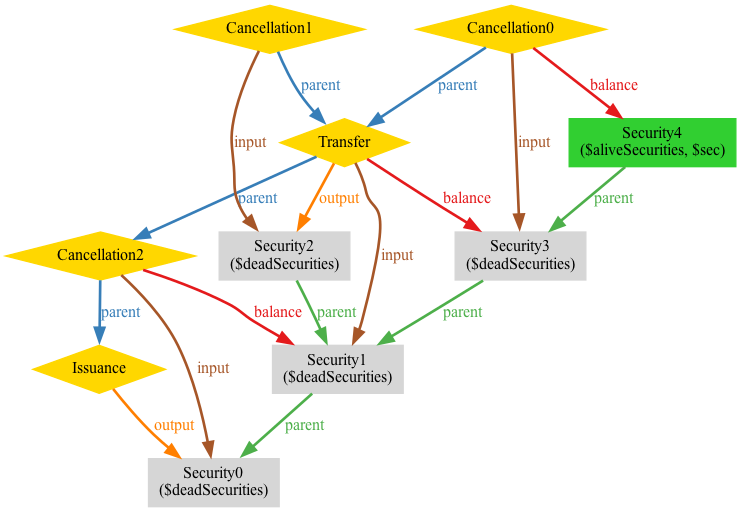
\includegraphics[width=0.9\textwidth]{images/spine.png}}
	\caption{A long chain of \glspl{transaction} arising from a single issuance}\label{fig:tt-alloy-example-transaction-single-issuance}
\end{figure}

In this instance, a security, denoted as \verb|Security$0|, was initially issued and subsequently partially cancelled. This cancellation resulted in the creation of a new security, referred to as \verb|Security$1|, which represents the remaining balance. Furthermore, a partial transfer of \verb|Security$1| led to the generation of two distinct securities, namely \verb|Security$3| and \verb|Security$4|, serving as the output and balance, respectively. Securities \verb|Security$2| and \verb|Security$3| are subsequently cancelled, while \verb|Security$4| is established as the balance \gls{security} to compensate for the cancellation of \verb|Security$3|.

\section{Discussion}

What we achieved by formalizing a model for the transactions that make up a company's capitalization table? First, we get a clear graphical view of the transactions. This allows one to analyze any sequence of transactions quickly, which is useful in auditing, for example. The graphical view also helps to communicate the business rules itself. Second, a system built upon our model would respect important conceptual, structural and accounting considerations that required in a correct design.

We know that the instances we presented as examples are consistent because if they weren't Alloy would respond with a failure to find any model. They are correct insofar our specification, and understanding of the problem is correct; our development of the model is based on extensive industry experience by the author\footnote{Prior to working in technology, both in academia and industry, the author held a BS in Economics and worked in Venture Capital funds and startups. Currently, the author owns a company that provides cap table management services}.

\section{Conclusion}

Alloy has been used in a wide range of applications in software engineering, database design, \gls{security} analysis~\cite{Carpio2021}\cite{Chen2006}, multiagent negotiations~\cite{Podorozhny}. It has also been applied to modeling beyond computer science, such as a model for central bank policy~\cite{Johnson2021}. A model of the same-origin-policy used in web browsers can be found in the 500 Lines or Less open-source book~\cite{500Lines19:online}.
%
There is a lack of existing models of \glspl{capitalization-table} in Alloy, as well as an absence of semantic models for this particular domain.

By using Alloy, we have been able to model the \gls{capitalization-table} of a company, and to show how a long chain of \glspl{transaction} could be rigorously modeled in a verifiable, auditable manner, in a way that was not possible within the original JSON Schema implementation.
%
We started with a \textit{data} specification and worked towards a \textit{domain} specification. The syntactical nature of the original \textit{data} model was enriched with a \textit{semantic} nature of the \textit{domain} behavior, taking into account the relationships between various types of entities and expected invariants (based on domain knowledge).

As a result, our model features a transaction tracing system that can be used to track the lineage of \glspl{security} and \glspl{transaction} in a company's capitalization table. We also showed how the model can be used to verify the consistency of the capitalization table, and to check that the accounting identities hold.

Future improvement is possible by:

\begin{itemize}
    \item Incorporating additional knowledge domain aspects by specifying the logical components of Vesting and Convertible Securities.
    \item Incorporating temporal features.
    \item Exploring the potential usage of the Alloy application programming interface (API) for the purpose of feeding real data to the system as predicates and testing if they are consistent.
\end{itemize}

Finally, the semantics of the rules we modeled are ultimately defined in legal documents. The model is a first step towards a more general formalization of business contract rules, which can be used to reason about the rules, and to verify that the rules are implemented correctly in software systems.